\chapter{Single-Cell System Performance Analysis under Correlated Shadow Fading}\label{ch:3}
\par Shadow fading has been proven to be a significant contributor to channel variations in wireless communication. In most cases shadow fading is assumed to have a log-normal fading distribution to model the loss at a certain location. However, in a mobile network, it is also important to know how shadow fading is correlated both in space and in time, which can greatly affect application layer behavior and service quality. This chapter is an attempt to characterize shadow fading so as to accurately study its impact on the application layer quality of service. If the correlation is strong over time and space, shadow fading can result in a long outage. In this chapter, we assume shadow fading is exponentially correlated in space. To study correlated shadow fading and its resultant outage durations, a first-order Markov chain model is developed and validated. The Markov chain model is constructed by partitioning the entire shadow fading range into a finite number of intervals. The state transition matrix of the Markov chain is derived from the joint probability distribution of correlated log-normal shadow fading. Based on the proposed Markov chain model, the frequency and duration of outage near the edge of a single cell is analyzed. To validate the Markov chain model, correlated Gaussian random fields are simulated to analyze the outage frequency and durations due to correlated shadow fading. Comparing the simulation results with the Markov chain model results, we can conclude that the proposed Markov chain model is an efficient way to describe the channel variations, and the user experienced outage behavior of the channel.
\section{Background}
In the past few decades, fading in wireless communication systems has been studied extensively in the literature. Fading phenomena can substantially affect the performance of a wireless communication system. In general, fading can be divided into two categories: large-scale fading and small-scale fading. A signal transmitted from source to destination will experience both large-scale and small-scale fading. Small-scale fading is caused by multipath propagation. Large-scale fading, which is also known as shadow fading, is caused by obstacles (trees, buildings, etc.) in the propagation path. Shadow fading is approximated by an independent log-normal distribution \cite{rappaport1996wireless} in most cases. Researchers have also shown that shadow fading is spatially correlated at different positions on the propagation path \cite{gudmundson1991correlation}, \cite{zhang2008novel}. The spatial correlation of shadow fading is important when studying the quality of service of a mobile system since it will result in long-lasting outage durations, which will deteriorate the performance of the applications running on the network. For example, in Figure \ref{building2}, the user is moving behind a row of tall buildings which block the signals from the base station. These tall buildings result in deep shadow fading, and the shadow fading of different positions behind these buildings are closely correlated.
\begin{figure}
\centering
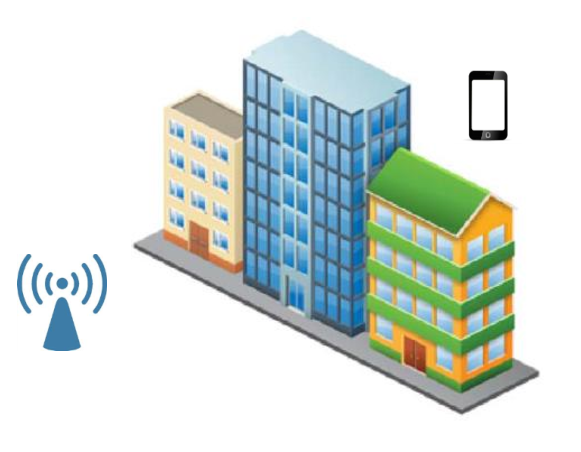
\includegraphics[width=9cm]{building.eps}
\caption{An example of building blockage.}
\label{building2}
\end{figure}
\par The spatial correlation of shadow fading has been investigated by numerous researchers. Based on empirical measurements, different autocorrelation models have been proposed for different scenarios and radio frequencies \cite{gudmundson1991correlation, sorensen1998correlation, weitzen2002measurement}. Szyszkowicz et al. \cite{szyszkowicz2010feasibility} studied shadow fading correlation models and investigated the feasibility of all these models. Among all these models, the analytical model proposed by Gudmundson \cite{gudmundson1991correlation} based on empirical measurements of $900MHz$ frequency is the one which is widely used in channel estimation. This model shows that shadow fading can be modeled as a first-order autoregressive process AR(1), which indicates a spatial exponential decaying autocorrelation function. Given this model, we propose a Markov chain model that can be constructed to capture the variation of shadow fading. The Markov chain models can in turn be used to accurately model the impact of shadow fading on higher layer protocols and applications. Since the shadow fading statistically follows a log-normal distribution, we can divide the entire range of shadow fading, which is $[-\infty,+\infty]$ into a finite number of intervals. Each interval is considered as a state of the Markov chain model. When the shadow fading falls in a particular interval, it is assigned to be in this particular state. The number of intervals (states) defines the granularity of the Markov chain model. The higher the number of states, the higher the precision in modeling the shadow fading. Correlated log-normal shadow fading has different variances with regard to different scenarios. For example, urban and suburban areas have different standard deviations based on empirical measurements. Different standard deviations of the log-normal shadow fading will result in different state transition matrices of the Markov chain model.
\par Outage events happen when the channel state is poor, and the received signals are not strong enough for the receiver to decode. Outage probability and the length of outage duration are important performance measurements of a wireless communication system over fading channels. Considering the applications which require low latency where buffer size is small, a long outage duration will drop the connection and lower the quality of service. To study the outage behavior of a communication system under correlated shadow fading, a well designed Markov chain model is a powerful tool. With a Markov chain model, the channel state in the next user position can be estimated from the current channel state given the current user position. Therefore, the system performance can be evaluated efficiently. Fading is a significant factor which causes dramatic channel state variations. Correlated shadow fading will result in long-lasting outage durations which is harmful to delay-sensitive real-time application and result in loss of quality of service. The Markov chain model can be used to analyze the probability distribution of outage events. The distribution and behavior of outage events will provide us the necessary information to improve wireless communication systems further. For example, efficient cooperative communication schemes can be designed to mitigate the outage behavior.
\par The main focus of this chapter is how to design a first-order Markov chain model to reflect the spatial correlation of shadow fading, and the study of outage behavior of a single cell wireless communication system given correlated shadow fading. The key contributions of this chapter are summarized below.
\begin{itemize}
\item Constructed a Markov chain model based on correlated shadow fading.
%\item Studied the proper number of states of the Markov chain model and validated it through simulation. \reminder{this is not a contribution since you just tried several options}
\item Analyzed the outage frequency and outage duration of a single cell wireless communication system over correlated shadow fading.
\end{itemize}
 The remaining sections of this chapter are organized as follows. The channel model with spatial correlated shadow fading is described in Section~\ref{sec:shadowing}. Section~\ref{sec:markov} shows how to construct the Markov chain model from the correlated shadow fading. Analysis of outage behavior is demonstrated in Section~\ref{sec:outage}. Simulation to validate the Markov chain model is illustrated in Section~\ref{sec:simulation}. Section~\ref{sec:conclusion} summarizes and concludes the chapter.
\section{Channel Model with Correlated Shadow Fading}
\label{sec:shadowing}
\begin{figure*}
\centering
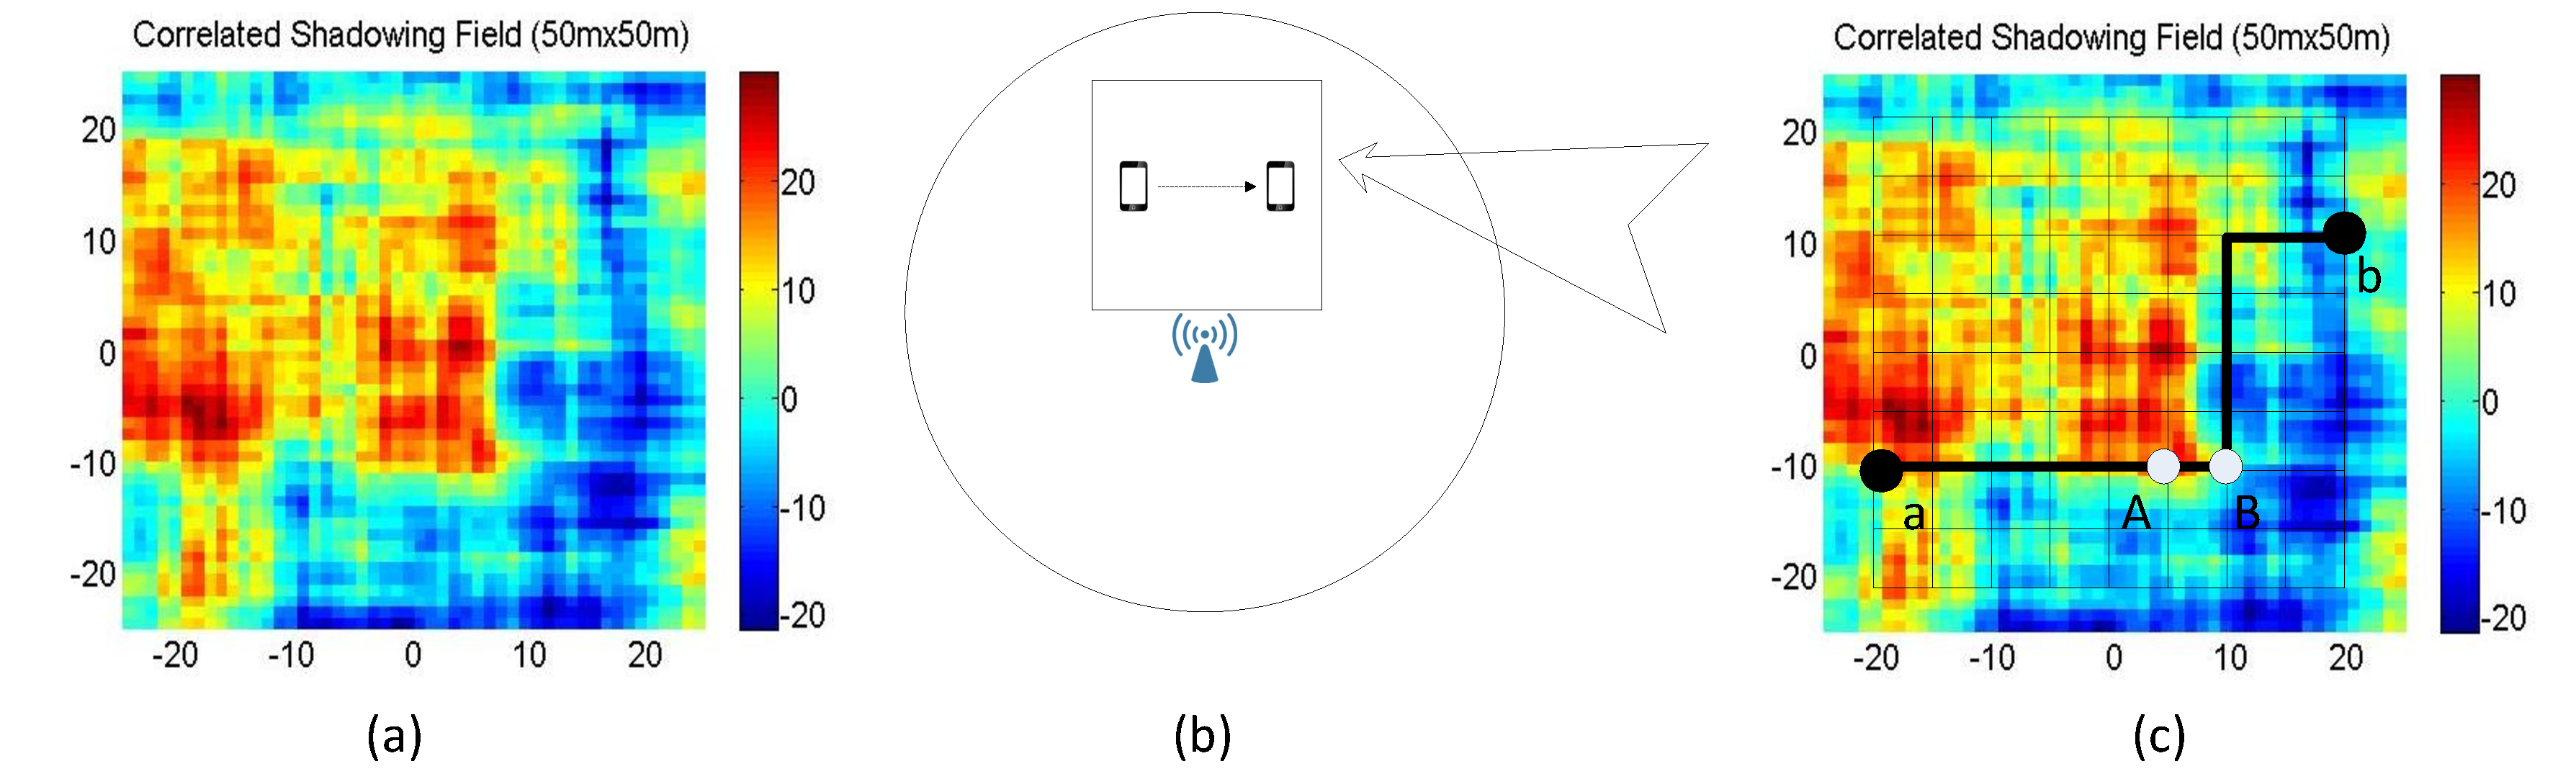
\includegraphics[width=14cm]{finalsystemab_V3.eps}
\caption{(a) A typical exponential correlated shadow fading field in a $50m\times50m$ area. The color bar denotes the value of the shadow fading in dB. (b) A single cell model with a MS moving on a fixed trajectory. (c) A locally generated correlated shadowing field for a fixed trajectory from point a to point b.}
\label{systemmodel}
\end{figure*}
To simplify the problem, we consider a single 4G LTE cell without any intercell interference in Figure \ref{systemmodel}(b). Due to the high bandwidth of OFDM systems,  LTE networks are more resilient to frequency selective fading \cite{rappaport1996wireless}, therefore in this chapter small-scale fading is ignored and shadow fading becomes the most important fading factor. There is a Base Station(BS) at the center of the cell. A Mobile Station (MS) is moving on a certain trajectory within the cell. The received signal on a link $(S\to D)$ between source and destination is given by:
\begin{equation}
y_{D} = G_{SD}x_{S}+n_{D}.
\end{equation}
where $x_{S}$ is the signal transmitted by the source and $y_{D}$ is the signal received by the destination. $n_{D}\sim \mathcal{CN}(0,N_{0})$ is additive white Gaussian noise. $G_{SD}$ is the channel gain from source to destination including path loss and shadow fading.  $\text{SNR} \triangleq P*G_{SD}^{2}/N_{0}$, is the end-to-end received signal-to-noise ratio (SNR). The destination successfully receives the signals if no outage event happens, i.e., $\log_{2}(1+\text{SNR})\ge R$, where $R$ is the required data rate. From the definition of SNR, no outage event happens as long as $G_{SD}^2 > \beta$, where $\beta = \frac{(2^{R}-1)*N_{0}}{P}$. Therefore the channel gain from transmitter to receiver determines if an outage will occur.
\par Here we rewrite the channel gain in the following form: $G_{dB}=PL(d)+S$, where $G_{dB}$ is $G_{SD}$ in $dB$, $PL$ denotes the propagation pathloss in $dB$, $d$ is the distance from BS to MS and $S$ denotes shadow fading factor. In most cases, shadow fading is modeled as an independent log-normal distribution \cite{goldsmith2005wireless} with a standard deviation derived from empirical measurements. In this model, the probability distribution of pathloss $G_{dB}$ is given by:
\begin{equation}
p(G_{dB})=\frac{1}{\sqrt{2\pi}\sigma_{G_{dB}}}exp[-\frac{(G_{dB}-\mu_{G_{dB})^2}}{2\sigma_{G_{dB}}^2}].
\end{equation}
where $\mu_{G_{dB}}$ is the average pathloss which is equal to $PL(d)$ and $\sigma_{G_{dB}}$ denotes the standard deviation of pathloss. Since shadow fading is the only fading factor that is considered here, $\sigma_{G_{dB}}$ is determined by the standard deviation of shadow fading.
This model fails to capture the spatial correlations in shadow fading. For examples, in Figure \ref{systemmodel}(c), shadow fading factors of two close positions A and B, which are $S_{A}$ and $S_{B}$, are not independent but correlated to each other. Empirical measurements showed that shadowing has significant correlations in several realistic scenarios and the correlated shadow fading can affect system performance \cite{graziano1978propagation}. Among all models derived from empirical measurements for correlated shadow fading, exponentially decaying correlation \cite{gudmundson1991correlation} is widely used. In this chapter, we choose this model to do further analysis. Figure \ref{systemmodel}(a) is an example of exponentially correlated shadowing field which is generated from the Graziano model \cite{graziano1978propagation}. This figure shows a $50\times50 m^{2}$ shadow fading area and illustrates that deep shadowing area is clustered and correlated (the blue area).
\par In Figure ~\ref{systemmodel}(c), the entire space is discretized. The MS moves on the lattice as shown. $A$ and $B$ are two neighbouring points. Assume the shadow fading (in dB) is $N(0,\sigma^{2})$ where $\sigma$ is the standard deviation, the spatial correlation between $S_{A}$ and $S_{B}$ will be given by
\begin{equation}
\rho_{A,B}=\frac{E[S_{A}S_{B}]}{\sigma^{2}}=e^{{-\frac{d_{A,B}}{d_{0}}}}
\end{equation}
where $d_{A,B}$ is the distance between $A$ and $B$, $d_{0}$ denotes the de-correlation distance \cite{bertoni1999radio}, which means if the distance between two points are substantially greater than $d_{0}$, the two shadow fading will be independent to each other. $d_{0}$ is determined by the environment, therefore urban and suburban areas have different de-correlation distances. An exponential correlation implies the shadow fading samples can be written as an AR(1) process as follows \cite{wei1994time}:
\begin{equation}
S_{B} = \rho S_{A} + (1-\rho)n_{A}
\label{e3}
\end{equation}
where $n_{A}$ denotes the channel noise at $A$. From this we conclude that the next channel state can be determined from the current channel state and the distance MS moves.
\section{Markov Chain Model}
\label{sec:markov}
In this section, we will construct a Markov chain model for exponential correlated shadow fading. First of all, we will discretize the space. In Figure \ref{systemmodel}(c), the space was partitioned into unit square spaces of $5\times5m^{2}$ (This granularity is used to describe the Markov chain model while in the simulation we uses a finer granularity). The MS moves on the lattices from point to point, the distance between each two neighboring points are considered as a unit distance $\delta d$. We prove that shadow fading factors of any two points that can be connected by a trajectory having jointly Gaussian distribution.
\begin{lem}
\emph{Exponential correlated shadow fading factors of any two points that can be connected by a trajectory have a jointly Gaussian distribution.}
\end{lem}
\begin{proof}Suppose the two points are $a$ and $b$, since there exists a trajectory connecting $a$ and $b$ like in Figure \ref{systemmodel}(c), we can assume there are $n$ positions on this trajectory $(t_{1},t_{2},\dots,t_{n})$. Then follow equation (\ref{e3}), we have the following:
\begin{equation}
\label{e5}
\begin{split}
S_{b} &=\rho S_{t_{n}}+(1-\rho)n_{t_{n}}\\
&=\rho(\rho S_{t_{n-1}}+(1-\rho)n_{t_{n-1}})+(1-\rho)n_{t_{n}}\\
&=\ldots\ldots\\
&=\rho^{n}S_{t_{1}}+\sum_{i=1}^{n}\rho^{n-i}(1-\rho)n_{t_{i}}\\
&=\rho^{n+1}S_{a}+\rho(1-\rho)n_{a}+\sum_{i=1}^{n}\rho^{n-i}(1-\rho)n_{t_{i}}
\end{split}
\end{equation}
Let $X=\alpha S_{a}+\beta S_{b}$, from equation ~\ref{e5}, the following can be derived:
\begin{equation}
X=\alpha S_{a}+\beta(\rho^{n+1}S_{a}+\rho(1-\rho)n_{a}+\sum_{i=1}^{n}\rho^{n-i}(1-\rho)n_{t_{i}})
\end{equation}
Since $S_{a}$, $n_{t_{i}}$ and $n_{a}$ are all independent and Gaussian random variables, we conclude that $X$ is also Gaussian, which implies that $S_{a}$ and $S_{b}$ are jointly Gaussian.
\end{proof}
\par Given the above conclusion, a Markov chain model can be constructed as follows:
\begin{itemize}
\item Divide the entire shadow fading range $[-\infty,+\infty]$ into a finite number of intervals $\{[-\infty,S_{0}],[S_{0},S_{1}],\dots,[S_{N},+\infty]\}$. Each interval represents a state of the Markov chain model.
\item Derive the state transition matrix of the Markov chain model from the probability distribution of the correlated shadow fading.
\item Derive the steady-state probability from the state transition matrix of the Markov chain model.
\end{itemize}
\par To derive the state transition matrix of the Markov chain model, we first investigate the probability density function of the correlated shadow fading. Since we have discretized the entire space into unit distances, here the state transition probability from point $A$ to point $B$ will be defined and used to calculate the state transition matrix of the Markov chain. Since $S_{A}$ and $S_{B}$ are jointly Gaussian with a correlated coefficient $\rho_{0}$, according to \cite{papoulis2002probability}, we have
\begin{equation}
\begin{split}
& f_{S_{A}|S_{B} =s_{B}}(s_{A}) =\frac{f_{S_{A},S_{B}}(s_{A},s_{B})}{f_{S_{B}}(s_{B})}\\
&=\frac{1}{\sigma_{A}\sqrt{2\pi(1-\rho_{0}^{2})}}\exp\{-\frac{(s_{A}-(\mu_{A}+\sigma_{A}\rho_{0}(s_{B}-\mu_{B})/\sigma_{B}))}{2\sigma_{A}^{2}(1-\rho_{0}^{2})}\}
\end{split}
\end{equation}
where $\mu_{A}$ and $\mu_{B}$ are expectations of log-normal shadow fading $S_{A}$ and $S_{B}$, which is typically set to $0$, while $\sigma_{A}$ and $\sigma_{B}$ are standard deviations, which are assumed to be equal to $\sigma_{0}$. Based on these assumptions, we can rewrite the equation as follows:
\begin{equation}
f_{S_{A}|S_{B} =s_{B}}(s_{A}) =\frac{1}{\sigma_{0}\sqrt{2\pi(1-\rho_{0}^{2})}}\exp\{-\frac{s_{A}-\rho_{0}s_{B}}{2\sigma_{0}^{2}(1-\rho_{0}^{2})}\}
\end{equation}
Assume there are $N$ states of the Markov chain model $ST_{1}, ST_{2},\cdots, ST_{N}$ where $ST_{i}$ corresponds to the interval $(S_{i-1}, S_{i}]$. Then we have the state transition probability as follows:
\begin{equation}
\label{statetransition}
\begin{split}
P_{i,j} &= P(S_{A}\in ST_{j}|S_{B}\in ST_{i})\\
&=\frac{P(S_{A}\in ST_{j}, S_{B}\in ST_{i})}{P(S_{B}\in ST_{i})}\\
&=\frac{\int_{S_{i-1}}^{S_{i}}(\int_{S_{j-1}}^{S_{j}}f_{(S_{A}|S_{B}=s_{B}}(s_{A})ds_{A})f(s_{B})ds_{B}}{\int_{S_{i-1}}^{S_{i}}f(s_{B})ds_{B}}
\end{split}
\end{equation}
From equation (\ref{statetransition}), the state transition matrix of the Markov chain can be derived. The steady-state transition matrix can be determined by $P$.
\section{Analysis of Outage Behavior}
\label{sec:outage}
In this section we analyze the outage behavior of the communication system using the Markov chain model of correlated shadow fading. The outage duration of a system is a significant factor influencing system performance. Given a fixed mobile trajectory, the Markov chain model described in Section \ref{sec:markov} provides an efficient way to study the outage events. In Figure \ref{systemmodel}(c), a fixed trajectory is given from point $a$ to $b$ through several intermediate points. Considering two consecutive points $A$ and $B$, we have $G_{A}=PL_{A}(d_{A})+S_{A}$ and $G_{B}=PL_{B}(d_{B})+S_{B}$ in $dB$. The probability that $A$ and $B$ are both in an outage area can be written as:
\begin{equation}
\begin{split}
&P(G_{A}<\gamma, G_{B}<\gamma) \\
&= P(S_{A}<\gamma-PL_{A}(d_{A}), S_{B}<\gamma-PL_{B}(d_{B}))
\end{split}
\end{equation}
%\begin{figure}
%\centering
%\includegraphics
%\caption
%\label{trajectory}
%\end{figure}

If $S_{A}<\gamma-PL_{A}(d_{A}) \in ST_{i}$ and $S_{B}<\gamma-PL_{B}(d_{B}) \in ST_{j}$, we can infer that, to avoid outage, the lower bound of the shadow fading factor $S_{A}$ is in state $ST_{i}$ and for $S_{B}$ is in state $ST_{j}$. State $ST_{i}$ and $ST_{j}$ are called lower bound states. Based on this approximation, the above probability can be written as:
\begin{equation}
P(G_{A}<\gamma, G_{B}<\gamma)=\sum_{m=0}^{i}\sum_{n=0}^{j} P(ST_{m})\bullet P(ST_{m},ST_{n})
\end{equation}
where $P(ST_{m})$ is the probability that $S_{A}$ is in the range of $ST_{m}$ which can be calculated from the Gaussian distribution. $P(ST_{m},ST_{n})$ can be found from the state transition matrix. Following this, the probability of an outage duration of length $l>L$ can be derived in below:
\begin{equation}
\begin{split}
&P(G_{1}<\gamma,\dots,G_{L}<\gamma)=\\
&\sum_{m_{1}=0}^{M_{1}}\dots\sum_{m_{L}=0}^{M_{L}} P(ST_{m_{1}})\bullet P(ST_{m_{1}},ST_{m_{2}})\\
&\bullet\dots\bullet P(ST_{m_{L-1}},ST_{m_{L}})
\end{split}
\end{equation}
where $M_{i}$, $i\in\{1,\dots,L\}$ are corresponding lower bound states of each position on the trajectory.


% \begin{table*}
% \begin{equation}
% P=\begin{bmatrix}
% \begin{smallmatrix}
% 0.5580 & 0.3627 & 0.0757 & 0.0036 & 3.5243\times10^{-5} & 0 & 0 & 0 \\
% 0.1587 & 0.4404 & 0.3359 & 0.0624 & 0.0026 & 2.3466\times10^{-5} & 0 & 0 \\
% 0.0184 & 0.1788 & 0.4546 & 0.2980 & 0.0484 & 0.0018 & 1.4485\times10^{-5} & 0 \\
% 0.0007 & 0.0258 & 0.2165 & 0.4624 & 0.2573 & 0.0361 & 0.0012 & 8.4341\times10^{-6} \\
% 8.4341\times10^{-6} & 0.0012 & 0.0361 & 0.2573 & 0.4624 & 0.2165 & 0.0258 & 0.0007 \\
% 0 & 1.4485\times10^{-5} & 0.0018 & 0.0484 & 0.2980 & 0.4546 & 0.1788 & 0.0184 \\
% 0 & 0 & 2.3466\times10^{-5} & 0.0026 & 0.0623 & 0.3359 & 0.4404 & 0.1587 \\
% 0 & 0 & 0 & 3.5243\times10^{-5} & 0.0036 & 0.0757 & 0.3627 & 0.5580 \\
% \end{smallmatrix}
% \end{bmatrix}
% \label{matrix}
% \end{equation}
% \end{table*}
\begin{table*}
\begin{equation}
P=\begin{bmatrix}
P1\\
P2\\
P3\\
P4\\
P5\\
P6\\
P7\\
P8\\
\end{bmatrix}
\label{matrix}
\end{equation}
\end{table*}

\begin{equation}
\begin{split}
& P1=\begin{bmatrix}
0.5580 & 0.3627 & 0.0757 & 0.0036 & 3.5243\times10^{-5} & 0 & 0 & 0
\end{bmatrix}\\
& P2 = \begin{bmatrix}
0.1587 & 0.4404 & 0.3359 & 0.0624 & 0.0026 & 2.3466\times10^{-5} & 0 & 0 
\end{bmatrix}\\
& P3 = \begin{bmatrix}
0.0184 & 0.1788 & 0.4546 & 0.2980 & 0.0484 & 0.0018 & 1.4485\times10^{-5} & 0
\end{bmatrix}\\
& P4 = \begin{bmatrix}
0.0007 & 0.0258 & 0.2165 & 0.4624 & 0.2573 & 0.0361 & 0.0012 & 8.4341\times10^{-6}
\end{bmatrix}\\
& P5 = \begin{bmatrix}
8.4341\times10^{-6} & 0.0012 & 0.0361 & 0.2573 & 0.4624 & 0.2165 & 0.0258 & 0.0007
\end{bmatrix}\\
& P6 = \begin{bmatrix}
0 & 1.4485\times10^{-5} & 0.0018 & 0.0484 & 0.2980 & 0.4546 & 0.1788 & 0.0184
\end{bmatrix}\\
& P7 = \begin{bmatrix}
0 & 0 & 2.3466\times10^{-5} & 0.0026 & 0.0623 & 0.3359 & 0.4404 & 0.1587
\end{bmatrix}\\
& P8 = \begin{bmatrix}
0 & 0 & 0 & 3.5243\times10^{-5} & 0.0036 & 0.0757 & 0.3627 & 0.5580
\end{bmatrix}
\end{split}
\label{smallmatrix}
\end{equation}
\par In this section, we employ Monte-Carlo simulation to validate our Markov chain model. To start the simulation, a large number of correlated shadowing fields are generated. As shown in Figure \ref{systemmodel}(b) and (c), instead of generating shadowing fields for the entire cell, we pick up a MS trajectory and generated shadowing fields that covers that trajectory. In this chapter, we choose the urban environment as the case to study. In this case, the shadow fading and Markov chain parameters are set as in Table \ref{SystemConfig}. The standard deviation of shadow fading is chosen to be $8dB$ following \cite{szyszkowicz2010feasibility}. The number of states of the Markov chain is set to be $3*\sigma_{0}/n*2+2$, where $n=1,3,8$ is the size of each range (state) in $dB$ except the two above $3\sigma_{0}$. $n$ in this case represents different granularities in the area of $[-3\sigma_{0},3\sigma_{0}]$. The state transition matrices are calculated with regard to each $n$. For example, when $n=8$, the states of the Markov chain model are:
\begin{equation}
\begin{split}
[&(-\infty,-24],(-24,-16],(-16,-8],(-8,0],\\
&[0,8],[8,16),[16,24),[24,+\infty)]
\end{split}
\end{equation} and the state transition matrix is given in (\ref{matrix} and \ref{smallmatrix}).
\section{Simulation Results}
\label{sec:simulation}

\begin{table}
\centering
\caption{\label{SystemConfig}Simulation Configuration Parameters}

\begin{tabular}{|c|c|}

\hline

\multirow{2}{*}{Okumura-Hata Model} & BS Height: $100m$\\
& MS Height: $1m$\\
\hline
%Rayleigh Fading & Coherence Time: $100ms$\\
%\hline
\multirow{5}{*}{Correlated Shadow Fading}
& De-Correlation Distance $d_{0}$: $20m$\\
& Standard Deviation $\sigma_{0}$: $8dB$\\
\hline
\multirow{3}{*}{Markov Chain Model} & Number of States:\\
& 50, 18, 8\\
& ($3*\sigma_{0}/n*2+2$, $n=1, 3, 8$)\\
\hline
MS Trajectory & Unit Distance $\delta d$: $1m$\\
\hline
Shadowing Field & $50\times50m^{2}$\\
\hline
Radio Frequency & $f: 1024MHz$\\
\hline
BS Transmission Power & $P: 30dbm$\\
\hline
SNR Requirement & $10dB$\\
\hline
\end{tabular}
\end{table}

\par To validate our Markov chain models, the probability distributions of outage durations corresponding to MS trajectories of length $l>1m$ up to $l>9m$ are studied given different number of states. Since there is a trade-off between the number of states and the complexity of the simulation computation, the simulated results also provide us information about the proper granularity of the Markov chain model to most accurately approximate the real channel. The simulation also confirms that correlated shadow fading indeed can cause long-lasting outage durations. In our simulation, the MS moves on a straight track which is around $900m$ away from the BS. Let $l$ denote the outage duration in meters, Figure \ref{prob} shows the probability of $l>L$. Comparing the two cases: with and without correlation, we can conclude that correlated shadow fading can result in severe long-lasting outage durations. Take $L=5$ for example, the correlated case gives $P(l>L)=12\%$, while in the non-correlated case the probability is around $0\%$. This illustrates the correlation between shadow fading cannot be neglected in mobility models. The MS speed is approximately the same as pedestrian speed which is $1m/s$ (Since the edge length of the lattice is $1m$, the MS moves one grid (unit distance) every second). Assuming this, the user will experience an outage of more than $9$ seconds with a probability of $7\%$.
\par To find out the proper number of states of the Markov chain model, three different Markov chain models with different number of states are tested. Basically we divide the $[-3\sigma_{0},3\sigma_{0}]$ area with different granularity, which is represented by $n=1,3,8$. When $n=1$, the interval $ST_{i}$ except $(-\infty,S_{0}]$ and $[S_{N},+\infty)$ is $1dB$. The results showed in Figure \ref{prob} indicates that when $n=1$, the curve is close to the correlation curve, which means that the Markov chain model becomes a good approximation of the channel to study the outage behavior of the system. Generally, more Markov states lead to more precise models. When the interval $[S_{i},S_{j}]$ becomes relatively large with regarding $\sigma_{0}$, the Markov chain model will fail to be a useful tool to study the outage behavior of the system. For example, in Figure \ref{prob}, when $n=8$, $P(l>1)$ is almost twice the correct $P(l>1)$. The prediction of the outage behavior of the system is not precise and useful anymore.
\begin{figure}
\centering
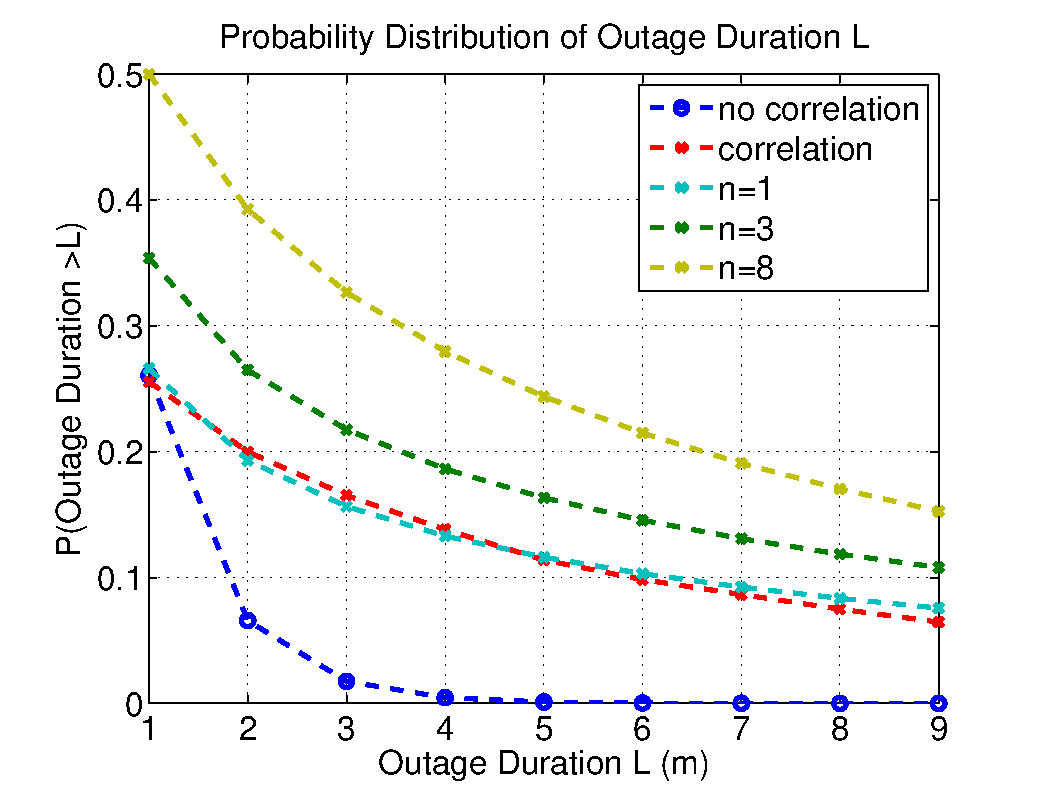
\includegraphics[width=12cm]{result_Plot_new.eps}
\caption{Probabilities of outage duration greater than $L$.}
\label{prob}
\end{figure}

\section{Conclusions}
\label{sec:conclusion}
\par In this chapter we investigated how shadow fading at different positions in a cellular network is correlated. In an environment where the correlation is high, shadow fading will result in long-lasting outage durations which can lead to a significant deterioration in system performance. To model spatially correlated shadow fading we divided the entire range of shadow fading into a finite number of intervals. A Markov chain model is then constructed, where each interval becomes a state of the Markov chain model. This model can be used to analyze the  outage behavior at the application layer. We demonstrated that a well designed Markov chain model with an appropriate number of states corresponding to the standard deviation of the shadow fading is indeed a powerful tool to study system performance. For a single-cell system, this Markov chain model is able to analyze the system performance because there only exist autocorrelation in this scenario. In next chapter, we will investigate the system performance of a multi-cell communication system. This model will not be capable to describe the scenario there. We will run simulations to show the system performance of a multi-cell system under exponentially correlated shadow fading.
%In future work, we will use this model to study the impact of shadow fading at the transport and higher layers.
